\documentclass[11pt]{article}

\usepackage[a4paper,margin=1in]{geometry}
\usepackage{amsmath,amssymb,amsthm,mathtools}
\usepackage{tikz}
\usetikzlibrary{positioning,calc}
\usepackage{booktabs}
\usepackage{hyperref}
\usepackage{listings}
\usepackage{xcolor}

\hypersetup{
  colorlinks=true,
  linkcolor=blue!50!black,
  citecolor=blue!50!black,
  urlcolor=blue!50!black
}

\lstdefinelanguage{Lean}{
  morekeywords={namespace,abbrev,structure,where,inductive,def,axiom,theorem,by,Prop,Nat,Type,deriving,Repr,DecidableEq,Not,Exists,fun,exact,cases,simp,end},
  sensitive=true,
  morecomment=[l]{--},
  morecomment=[s]{/-}{-/},
  morestring=[b]"
}

\lstset{
  basicstyle=\ttfamily\small,
  breaklines=true,
  frame=single,
  columns=fullflexible,
  keywordstyle=\color{blue!60!black},
  commentstyle=\color{green!40!black},
  stringstyle=\color{orange!60!black}
}

\newtheorem{definition}{Definition}[section]
\newtheorem{proposition}[definition]{Proposition}
\newtheorem{corollary}[definition]{Corollary}
\newtheorem{remark}[definition]{Remark}

\title{Free Numbers:\\Local Quaternionic Closure and Global Residual Chart Normalization\\\large A Non-Collapsing Quaternionic Chart Algebra}
\author{Free Number Authors}
\date{Version v0.2-pre.2\\2026-06-21}

\begin{document}
\maketitle

\begin{abstract}
We introduce \textbf{free numbers}, a formal framework for representing local algebraic closures and their global residual composition without collapsing all local structures into a single ambient vector space. The construction begins with a local closure $F_1$, whose primitive fold plane is two-dimensional and whose completed local algebra is shown to be isomorphic to the real quaternion algebra $\mathbb H$. The global structure $F$ is then defined as a finite term system generated from a disjoint family of local closures, quotiented only by admissible equivalences that preserve local algebraic structure, boundary data, conjugation, and residual purity.

The central feature of the framework is the distinction between \textbf{admissible transitions}, which allow local charts to be identified, and \textbf{residual transitions}, which must not be collapsed. When two local elements cannot be compared by admissible transport, a new generated chart is introduced. This yields a residual chart network in which global composition need not be globally associative, but is instead tracked through finite generation histories.

We further define a Gen-normalization procedure and isolate a minimal rewriting kernel suitable for Lean-style formalization. The kernel includes finite terms, one-step reduction, reflexive-transitive reduction, normal forms, and a well-founded measure for a restricted core system. The purpose of the present paper is not to claim a completed semantic theory, but to provide a precise algebraic and rewriting core for non-collapsing relational state spaces in principle.
\end{abstract}

\tableofcontents

\section{Introduction}

Many formal models represent a system by embedding all states into a single global space. This is often convenient, but it can erase distinctions between locally valid structures that are not globally comparable. In particular, two local configurations may each possess a coherent internal algebra, while no admissible transition exists that preserves the relevant algebraic, boundary, and residual data between them.

This paper proposes \textbf{free numbers} as a formal response to this problem. The guiding idea is simple:
\[
\text{local closure should not imply global collapse.}
\]

The construction separates two levels.

First, a local closure $F_1$ is defined. At this level, the structure closes in a quaternionic form:
\[
F_1 \cong_{\mathbb{R}\text{-alg}} \mathbb{H}.
\]

Second, a global free-number structure $F$ is constructed from many local closures $F_{1,\alpha}$. These local charts are not identified merely because they are algebraically isomorphic. They may be identified only when an admissible transition preserves the required algebraic and boundary structure. Otherwise, their interaction generates a new chart.

Thus the global structure is not a single quaternion algebra. Rather, it is a finite term system of local quaternionic closures, admissible transports, residual boundaries, and generated charts.

Figure~\ref{fig:local-global-collapse} summarizes the central distinction.

\begin{figure}[t]
\centering
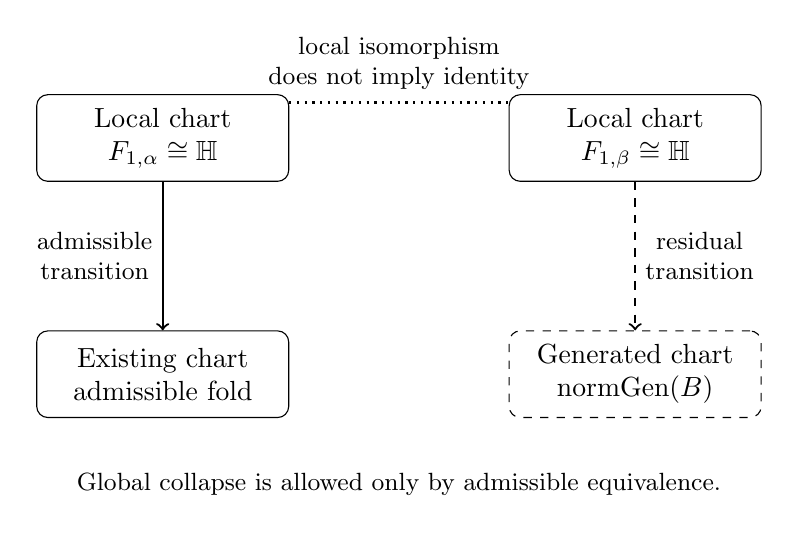
\begin{tikzpicture}[
  chart/.style={draw, rounded corners, minimum width=3.2cm, minimum height=1.1cm, align=center},
  gen/.style={draw, rounded corners, dashed, minimum width=3.2cm, minimum height=1.1cm, align=center},
  arrow/.style={->, thick},
  badarrow/.style={->, thick, dashed},
  note/.style={align=center, font=\small}
]

\node[chart] (A) at (0,0) {Local chart\\$F_{1,\alpha}\cong\mathbb H$};
\node[chart] (B) at (6.0,0) {Local chart\\$F_{1,\beta}\cong\mathbb H$};

\node[chart] (C) at (0,-3) {Existing chart\\admissible fold};
\node[gen] (D) at (6.0,-3) {Generated chart\\$\operatorname{normGen}(B)$};

\draw[arrow] (A) -- node[left, note] {admissible\\transition} (C);
\draw[badarrow] (B) -- node[right, note] {residual\\transition} (D);

\draw[thick, dotted] ([yshift=0.45cm]A.east) -- ([yshift=0.45cm]B.west);
\node[note] at (3.0,0.95) {local isomorphism\\does not imply identity};

\node[note] at (3.0,-4.4) {Global collapse is allowed only by admissible equivalence.};

\end{tikzpicture}

\caption{Local closure does not imply global collapse. A solid arrow denotes an admissible transition as described in Section~\ref{sec:admissible-transitions}; a dashed arrow denotes a residual transition as described in Section~\ref{sec:residual-transitions}. The generated chart is normalized rather than collapsed, reflecting the Gen-normalization procedure of Section~\ref{sec:gen-normalization}.}
\label{fig:local-global-collapse}
\end{figure}

\section{Informal Motivation}

The motivation for free numbers is the need to describe systems in which local algebraic consistency and global comparability are distinct notions.

A local chart may be internally closed. It may have a unit, conjugation, multiplication, and a norm-like self-consistency trace. However, two such charts may still fail to be globally equivalent. Their difference may not be an error to be removed, but a residual structure to be preserved.

In this sense, free numbers are designed to represent relational configurations where:
\begin{enumerate}
  \item local closure is meaningful;
  \item global identification is not automatic;
  \item residual mismatch must be tracked;
  \item new comparison charts may be generated by composition;
  \item normalization should not erase non-admissible differences.
\end{enumerate}

The framework is intentionally conservative. It does not assert that all residual structures have a single semantic interpretation. It only provides a formal language in which residual comparison failure is not immediately collapsed.

\section{Contributions}

The main contributions are as follows.
\begin{enumerate}
  \item \textbf{Local quaternionic closure.} We define a local closure $F_1$ and identify the algebraic form under which it is isomorphic to the real quaternion algebra $\mathbb H$.
  \item \textbf{Global residual chart construction.} We define a global free-number structure $F$ as a finite term system generated from a disjoint family of local closures:
  \[
  F = \operatorname{Term}_{\mathcal R}\left(\bigsqcup_{\alpha\in\mathcal B_0}F_{1,\alpha}\right)/\equiv_{\mathrm{adm}}.
  \]
  \item \textbf{Admissible versus residual transitions.} We distinguish transitions that preserve the required local structure from transitions whose residuals must be retained.
  \item \textbf{Generated charts.} We introduce a chart-generation operation for the interaction of locally closed but globally non-comparable elements.
  \item \textbf{Gen-normalization.} We formulate a normalization scheme that either folds generated charts into existing admissible charts or marks them as normalized residual charts.
  \item \textbf{Minimal formal kernel.} We provide a Lean-style rewriting core consisting of terms, reductions, reflexive-transitive reductions, normal forms, and a well-founded measure for a restricted system.
\end{enumerate}

\section{Scope and Non-Claims}

This paper does not claim that free numbers constitute a completed theory of meaning, time, cognition, or physical reality.

The present work is limited to the following claim:
\[
\text{free numbers provide a formal algebraic and rewriting framework for local closures connected by admissible and residual chart structure.}
\]

In particular, this paper does not assume:
\begin{enumerate}
  \item that all global products are associative;
  \item that all algebraically isomorphic local charts are identical;
  \item that residual transitions may be quotiented away;
  \item that scalar projections determine equality;
  \item that the local quaternionic form exhausts the global structure.
\end{enumerate}

The global structure $F$ is not identified with $\mathbb H$. Only the local closure $F_1$ is quaternionic.

The current Lean mini-kernel uses \texttt{Nat} tags for \texttt{Chart} and \texttt{LocalId}. These tags are provisional syntactic labels only. In particular, chart distinctness, disjoint-copy semantics, and boundary isomorphism are not yet enforced at the kernel level. The kernel proves termination of the restricted Gen-normalization core only; it does not yet formalize the full non-identical-copy semantics of
\[
\bigsqcup_{\alpha} F_{1,\alpha}.
\]
These components are deferred to later versions under chart-distinctness refinement, \texttt{BoundaryIso}, and \texttt{EqAdm}.

\section{Local Closure \texorpdfstring{$F_1$}{F1}}

We construct the local closure as an explicit associative algebra rather than
assuming a four-dimensional multiplication table in advance.

Let
\[
U=\operatorname{span}_{\mathbb R}\{u,v\}
\]
be a two-dimensional real vector space, and let $T(U)$ be its unital tensor
algebra. Let $I$ be the two-sided ideal generated by
\[
u^2+1,\qquad v^2+1,\qquad uv+vu.
\]
Define
\[
\boxed{F_1:=T(U)/I.}
\]
Because $T(U)$ is associative and $I$ is a two-sided ideal, $F_1$ is a unital
associative real algebra. In the quotient,
\[
u^2=v^2=-1,\qquad uv=-vu.
\]
This is the real Clifford algebra $\mathrm{Cl}_{0,2}$ in a two-generator
presentation. Set
\[
I:=u,\qquad J:=v,\qquad K:=uv.
\]
Only $u,v$ are primitive generators; $K$ is their product.

\begin{proposition}[Spanning form]
Every element of $F_1$ is a real linear combination of
\[
1,\qquad u,\qquad v,\qquad uv.
\]
Hence $\dim_{\mathbb R}F_1\le4$.
\end{proposition}

\begin{proof}
Use $vu=-uv$ to move every $u$ to the left of every $v$, then use
$u^2=v^2=-1$ to reduce both exponents modulo two. Every word reduces, up to
sign, to one of $1,u,v,uv$.
\end{proof}

\begin{proposition}[Local quaternionic form]
\[
\boxed{
F_1=T(U)/(u^2+1,\ v^2+1,\ uv+vu)
\cong_{\mathbb R\text{-alg}}\mathbb H.
}
\]
\end{proposition}

\begin{proof}
Define a unital algebra homomorphism $\phi:T(U)\to\mathbb H$ by
$\phi(u)=i$ and $\phi(v)=j$. The generators of $I$ lie in $\ker\phi$, so
$\phi$ descends to a surjection
\[
\overline\phi:F_1\longrightarrow\mathbb H.
\]
Its image contains $1,i,j,ij=k$, hence $\dim_{\mathbb R}F_1\ge4$.
The spanning proposition gives the reverse inequality, so the surjection is an
isomorphism.
\end{proof}

The third pure direction is the product $uv$, equivalently the bivector
direction in $\Lambda^2U$. This local theorem does not identify different
local copies globally; global chart identity remains a separate rule.

\section{Local Charts and Non-Identical Copies}

Let $\mathcal B_0$ be a family of initial local chart labels. For each $\alpha\in\mathcal B_0$, let
\[
F_{1,\alpha}=\operatorname{span}_{\mathbb R}\{e_{0,\alpha},I_\alpha,J_\alpha,K_\alpha\}.
\]
Each chart satisfies
\[
F_{1,\alpha}\cong_{\mathbb R\text{-alg}}\mathbb H.
\]
However, for $\alpha\neq\beta$, we do not identify $F_{1,\alpha}$ and $F_{1,\beta}$ merely because both are quaternionic. Instead, we begin with the disjoint union
\[
\widetilde F=\bigsqcup_{\alpha\in\mathcal B_0}F_{1,\alpha}.
\]
Thus two elements with the same coordinate expression in two different charts remain distinct unless an admissible equivalence is explicitly given.

\section{Admissible Transitions}
\label{sec:admissible-transitions}

A transition
\[
T_{\beta\alpha}:F_{1,\alpha}\to F_{1,\beta}
\]
is called \textbf{admissible} if it preserves the required local structure.

At minimum, an admissible transition must preserve:
\begin{enumerate}
  \item the distinguished local unit;
  \item local multiplication;
  \item conjugation;
  \item the local self-consistency trace;
  \item boundary data associated with chart generation.
\end{enumerate}

If such a transition exists, then elements may be identified under admissible equivalence:
\[
x_\alpha\equiv_{\mathrm{adm}}T_{\beta\alpha}(x_\alpha).
\]
The admissible equivalence relation is generated only by such structure-preserving transitions and by local algebraic laws.

Residual transitions are not included in admissible equivalence.

\subsection*{Operational criterion for admissibility}

In the present version, admissibility is treated as a structural condition rather than as a fully implemented decision procedure. A transition
\[
T_{\beta\alpha}:F_{1,\alpha}\to F_{1,\beta}
\]
is admissible only if it preserves all data required to regard the two local charts as the same chart for the purposes of the current construction.

Concretely, the intended admissibility criterion consists of the following preservation requirements:
\begin{enumerate}
  \item \textbf{unit preservation}:
  \[
  T_{\beta\alpha}(e_{0,\alpha})=e_{0,\beta};
  \]
  \item \textbf{multiplication preservation}:
  \[
  T_{\beta\alpha}(xy)=T_{\beta\alpha}(x)T_{\beta\alpha}(y);
  \]
  \item \textbf{conjugation preservation}:
  \[
  T_{\beta\alpha}(x^*)=T_{\beta\alpha}(x)^*;
  \]
  \item \textbf{local trace preservation}:
  \[
  Q_\beta(T_{\beta\alpha}(x))=Q_\alpha(x);
  \]
  \item \textbf{boundary preservation}, meaning that generated boundary data is mapped to boundary data with the same structural origin.
\end{enumerate}

The abstract predicate \texttt{ExistingBoundary} in the minimal Lean kernel should be read as a placeholder for the case where these preservation requirements have already been satisfied at the boundary level. It is not intended to identify charts merely because they are algebraically isomorphic.

A full decision procedure for admissibility, including boundary isomorphism and residual purity, is deferred to later versions.

\section{Residual Transitions}
\label{sec:residual-transitions}

A transition that fails to preserve the required data is called \textbf{residual}.

A residual transition is not an error. It is a record that two local closures cannot be collapsed without losing structure.

For a candidate transition $S_{\beta\alpha}$, one may define residual components such as
\[
\Delta_e^S,\quad \Delta_\cdot^S,\quad \Delta_*^S,\quad \Delta_Q^S.
\]
These respectively measure failure to preserve the unit, multiplication, conjugation, and local quadratic trace.

The collection
\[
\operatorname{Res}(S_{\beta\alpha})=(\Delta_e^S,\Delta_\cdot^S,\Delta_*^S,\Delta_Q^S)
\]
is called the residual signature of the candidate transition.

Only when the residual signature is pure, or can be reduced to a pure admissible transition by an explicitly allowed normalization, may the corresponding transition contribute to admissible equivalence.

\section{Global Free Numbers}

The global free-number structure is defined by finite generated terms modulo admissible equivalence:
\[
F=\operatorname{Term}_{\mathcal R}\left(\bigsqcup_{\alpha\in\mathcal B_0}F_{1,\alpha}\right)/\equiv_{\mathrm{adm}}.
\]
The term grammar includes:
\begin{enumerate}
  \item local atomic elements;
  \item formal products;
  \item conjugates;
  \item generated chart terms.
\end{enumerate}

Products are syntactic unless they occur inside a common local chart or can be reduced by admissible transport. In particular, global associativity is not assumed.

Thus $(XY)Z$ and $X(YZ)$ may represent different generation histories unless an admissible equivalence relates them.

\section{Generated Charts}

Given elements
\[
x_\alpha\in F_{1,\alpha},\qquad y_\beta\in F_{1,\beta},
\]
if no admissible comparison allows them to be multiplied inside a common existing chart, their interaction generates a new chart:
\[
\gamma=\operatorname{Gen}(\alpha,x;\beta,y).
\]
This operation does not merely create a value. It creates a new local context in which the interaction can be represented.

The boundary of the generated chart records its origin:
\[
\partial\gamma=(\alpha,x;\beta,y).
\]
Generated charts are therefore not identified solely by algebraic isomorphism. Their boundary data is part of their identity.

\section{Gen-Normalization}
\label{sec:gen-normalization}

Gen-normalization determines whether a generated chart can be folded into an existing admissible chart or must be retained as a new normalized residual chart.

The normalization procedure follows four informal rules.
\begin{enumerate}
  \item If the product is already local, compute locally.
  \item If admissible transport places the factors in a common chart, compute there.
  \item If the generated chart is admissibly equivalent to an existing chart, fold it into that chart and mark it normalized.
  \item Otherwise, retain it as a new normalized generated chart.
\end{enumerate}

The purpose of normalization is not to erase residuals. It is to prevent repeated unresolved generation while preserving non-admissible differences.

\section{Minimal Rewriting Kernel}
\label{sec:minimal-rewriting-kernel}

A minimal rewriting kernel can be isolated as follows.

Terms are generated by
\[
\operatorname{atom},\quad \operatorname{mul},\quad \operatorname{star},\quad \operatorname{gen},\quad \operatorname{normGen}.
\]
A one-step reduction relation $Red$ includes:
\begin{enumerate}
  \item local multiplication;
  \item folding a generated chart into an existing normalized chart;
  \item marking a fresh generated chart as normalized.
\end{enumerate}

In the restricted kernel, pure transport is temporarily excluded from $Red$ until a transport cost, a transport normality condition, or a separate preprocessing relation is introduced.

\subsection*{Why transport is excluded from the restricted kernel}

The relation \texttt{PureMove} represents admissible transport between local elements. It is declared in the Lean kernel but intentionally excluded from the restricted reduction relation $Red$.

The reason is technical. A transport step may preserve both
\[
openGenCount
\]
and
\[
termSize.
\]
If such a step were included without an additional decreasing measure, the restricted termination proof would no longer be immediate.

Future versions may restore transport in one of three ways:
\begin{enumerate}
  \item by assigning a \textbf{transport cost} that strictly decreases along admissible transport chains;
  \item by requiring a \textbf{transport normality} condition, so that transport is performed only as a preprocessing step;
  \item by separating transport from $Red$ and treating it as an equivalence-side operation rather than as a reduction step.
\end{enumerate}

In v0.2-pre.2, the goal remains deliberately narrower: to isolate a terminating Gen-normalization core before restoring the full transport system.

A lightweight measure is defined by the repeated-addition form
\[
weight(X)=openGenCount(X)+openGenCount(X)+termSize(X).
\]
This is mathematically equal to
\[
2\cdot openGenCount(X)+termSize(X),
\]
but the repeated-addition form matches the Lean kernel exactly and keeps the natural-number expression syntactically minimal. For the restricted kernel, every one-step reduction strictly decreases this measure:
\[
Red(X,Y)\Rightarrow weight(Y)<weight(X).
\]
This gives a well-founded core suitable for defining normal forms.

\section{Normal Forms}

Let $Red^*$ denote the reflexive-transitive closure of $Red$. A term $N$ is a normal form of $X$ if
\[
Red^*(X,N)
\]
and there is no term $Y$ such that
\[
Red(N,Y).
\]
Equivalently,
\[
NormalForm(N):=\neg\exists Y,\ Red(N,Y).
\]
The minimal kernel does not yet prove uniqueness of normal forms modulo admissible equivalence. That requires weak confluence and the full admissible equivalence relation.

\section{Deferred Proof: Weak Confluence}

The present version establishes a terminating restricted reduction kernel. In this restricted kernel, pure transport is not included in the one-step reduction relation $Red$. This allows the Gen-normalization core to be equipped with a simple well-founded measure.

Weak confluence modulo admissible equivalence is not required for the restricted termination result and is deferred to a later version. In the full system, weak confluence must account for the interaction among:
\begin{enumerate}
  \item local multiplication;
  \item admissible transport;
  \item existing-chart folding;
  \item fresh generated-chart normalization;
  \item admissible equivalence of boundaries;
  \item residual purity.
\end{enumerate}

The intended statement is that if
\[
X\to Y
\]
and
\[
X\to Z,
\]
then $Y$ and $Z$ can be reduced to terms $Y'$ and $Z'$ such that
\[
Y'\equiv_{\mathrm{adm}} Z'.
\]
This proof is deferred because it depends on the full admissible equivalence relation, boundary isomorphism, and residual purity criteria, which are outside the minimal kernel of the present version.

\section{Projection and \texorpdfstring{$\Gamma$}{Gamma}}

A scalar projection may be defined on normalized self-consistency traces, but projection must not create equality.

That is,
\[
\rho(X)=\rho(Y)
\]
must not imply
\[
X\equiv_{\mathrm{adm}}Y.
\]

A projection suitable for global magnitude comparison must satisfy at least:
\begin{enumerate}
  \item admissible invariance;
  \item local normality;
  \item non-constancy;
  \item residual sensitivity.
\end{enumerate}

A global magnitude defect may then be expressed as
\[
\Gamma_\rho^{\mathrm{mag}}(X,Y)=\frac{\rho(N_F^{\mathrm{norm}}(XY))}{\rho(N_F^{\mathrm{norm}}(X))\rho(N_F^{\mathrm{norm}}(Y))}.
\]
In local admissible sectors, one expects $\Gamma=1$. In residual sectors, $\Gamma\neq1$ may occur.

\section{Discussion}

Free numbers are designed to formalize a distinction that is often blurred: local closure is not the same as global identity.

The local quaternionic closure $F_1$ provides a compact algebraic core. The global structure $F$ then preserves the fact that many such local closures may coexist without being collapsible into one global space.

This gives a formal language for non-collapsing relational state spaces. It may be useful wherever comparison failure is structural rather than accidental.

The present construction may also admit possible extensions to residual-based reconstruction. Those topics are outside the scope of the present paper. Here we restrict attention to the algebraic and rewriting core of free numbers.

\section{Conclusion}

We have introduced free numbers as a formal structure built from local quaternionic closures, admissible transitions, residual signatures, generated charts, and Gen-normalization.

The key point is that local algebraic equivalence does not automatically imply global identification. Residual differences are retained unless an admissible transition justifies their collapse.

The resulting structure is neither a single quaternion algebra nor a conventional global vector space. It is a finite generated chart network with controlled normalization.

A minimal Lean-style rewriting kernel supports the claim that the restricted Gen-normalization core can be organized as a terminating reduction system. Future work includes the full formalization of admissible equivalence, residual purity, weak confluence, projection-sensitive invariants, and transport-normalized reductions.

\appendix
\section{Minimal Lean Kernel}

The following appendix contains the minimal rewriting kernel used to represent terms, one-step reductions, transitive reductions, normal forms, and a decreasing weight measure. This kernel is intentionally restricted: pure transport is not yet included in the reduction relation.

The termination theorem is proved relative to Lean's standard \texttt{propext} axiom together with the abstract relations \texttt{LocalMul}, \texttt{ExistingBoundary}, and \texttt{FreshBoundary}. Running
\begin{lstlisting}[language=Lean]
#print axioms FreeNumKernel.red_weight_decreases
\end{lstlisting}
is expected to list exactly these dependencies:
\begin{lstlisting}[language=Lean]
propext
FreeNumKernel.ExistingBoundary
FreeNumKernel.FreshBoundary
FreeNumKernel.LocalMul
\end{lstlisting}
The abstract relation \texttt{PureMove} is declared but excluded from \texttt{Red}, and is therefore not expected to appear in this dependency list.

\lstinputlisting[language=Lean]{../lean/Minimal.lean}

\section{Axioms and Deferred Components}

The present version separates proved components, definitional components, and deferred components. Table~\ref{tab:axioms} lists the abstract assumptions used in the minimal formal kernel and indicates their intended role in later versions. The dependency profile of \texttt{red\_weight\_decreases} is explicitly exposed rather than hidden: it is relative to \texttt{propext} and to the abstract relations A1--A3.

\begin{table}[h]
\centering
\small
\begin{tabular}{llll}
\toprule
Label & Component & Role & Status \\
\midrule
A1 & \texttt{LocalMul} & Local atom product & Abstract relation \\
A2 & \texttt{ExistingBoundary} & Fold into existing boundary & Abstract relation \\
A3 & \texttt{FreshBoundary} & Retain as normalized & Abstract relation \\
A4 & \texttt{PureMove} & Admissible transport & Excluded from \texttt{Red} \\
A5 & \texttt{BoundaryIso} & Boundary equivalence & Deferred \\
A6 & \texttt{ResidualPurity} & Residual purity criterion & Deferred \\
A7 & \texttt{EqAdm} & Admissible equivalence & Deferred \\
A8 & \texttt{WeakConfluence} & Normal form uniqueness modulo EqAdm & Deferred \\
A9 & \texttt{EffectiveMagProjection} & Residual-sensitive scalar projection & Deferred \\
A10 & \texttt{TransportNormalizedReduction} & Restore transport into reduction & Deferred \\
\bottomrule
\end{tabular}
\caption{Axioms and deferred components in v0.2-pre.2.}
\label{tab:axioms}
\end{table}

The minimal kernel proves only the following restricted claim:
\[
Red(X,Y)\Rightarrow weight(Y)<weight(X).
\]
This establishes termination for the restricted Gen-normalization core, not for the full admissible transport system. It is not a proof of weak confluence, global normal-form uniqueness, full admissible transport, or full chart-distinctness semantics.

\end{document}
